This thesis details a control method to perform setpoint regulation for a soft robotic actuator. The proposed method combines classic control theory with additional control methods to fit the purpose of controlling soft robots. This introductory chapter provides context in which this research is performed. First, a detailed description of soft robots is provided. Illustrations of already developed soft robots are included. Furthermore, parallels and differences are drawn between soft robots and classic rigid robots. This helps to understand the need for new control methodologies for solving control problems applied to soft robots. This chapter is concluded by detailing the research outline and its research objectives.


\section{Background}



\subsection{Introduction to soft robotics}

In recent years, the field of soft robotics has received a substantial increase of interest. Soft robots reshape the idea of using robots for industrial processes. Currently, rigid robots dominate the field of industrial automation. As they excel in accuracy, repeatability and load capacity. However, these robots tend to be unsafe to operate in human-centred environments. Classic robots are made from rigid material and accelerate to high velocities, creating a dangerous setting for humans. Additionally, these robots have limited degrees of freedom, making it harder to avoid obstacles. To evade the risks of potential harm, soft robots are made from flexible material. Furthermore, their inherently dexterous structure allows soft robots to move around obstacles. This makes soft robots robust in constantly changing environments. The foundation of soft robotic design is often found in nature. This includes inspiration for material, locomotion, and morphology. A few examples of bio-inspired soft robots include emulated trunks \cite{hannan2003kinematics} inspired by the proboscis of an elephant, robots based on the arm of octopus \cite{wang2013visual}, and robots that replicate the movement of fish \cite{marchese2014}. Figure (\ref{fig1:softexample}) shows a few experimental soft robots. 


\begin{figure}[H]       
    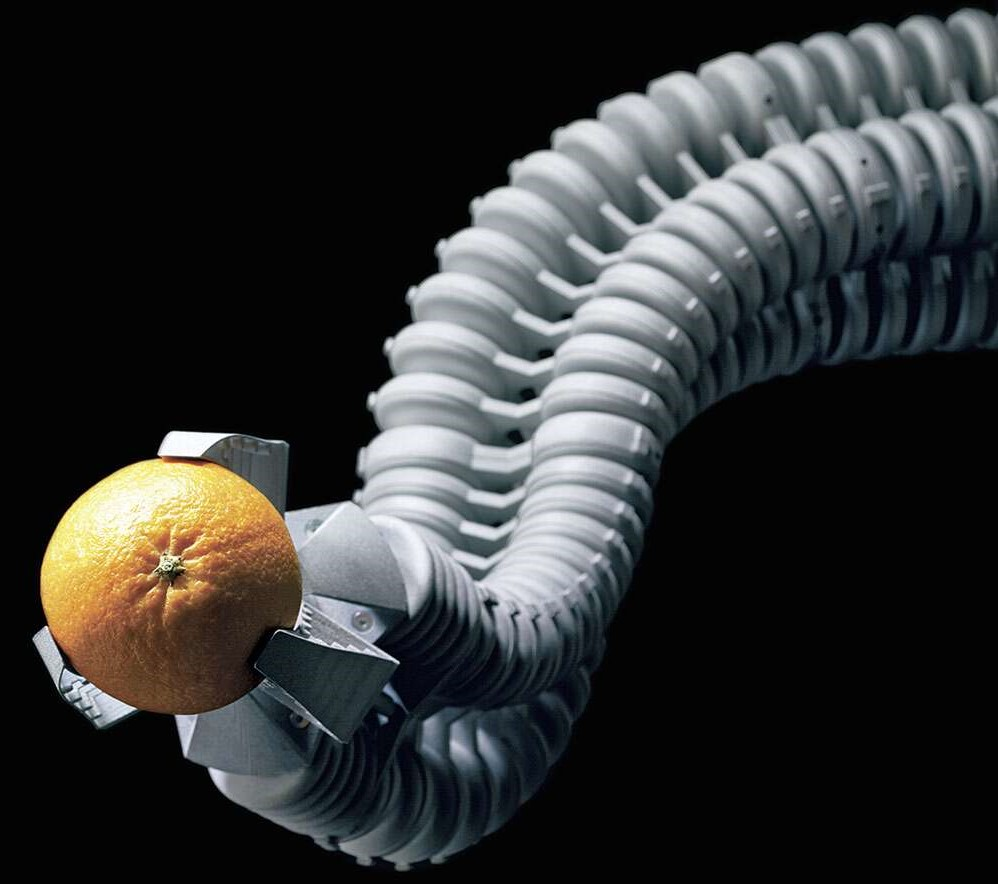
\includegraphics[width = 0.3\textwidth]{Figures/Introduction/bhasinasappel.jpg}   
    \hspace{0px}
    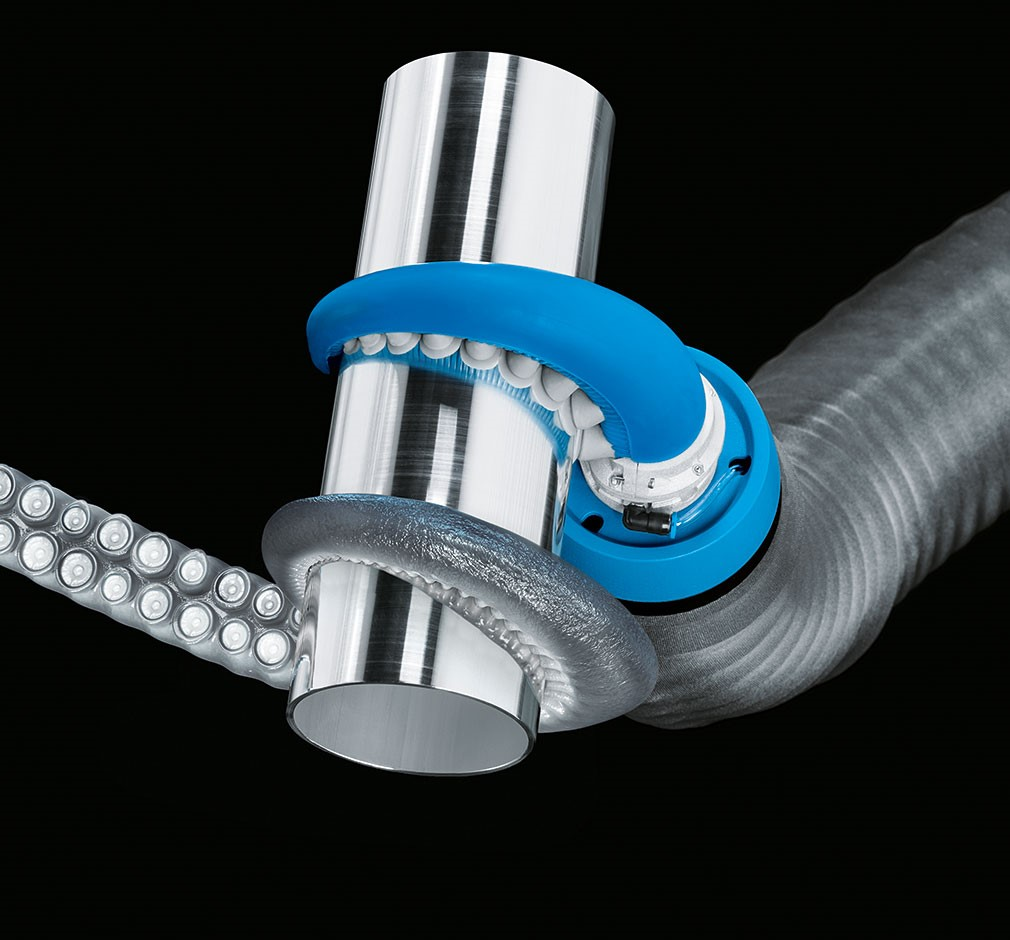
\includegraphics[width = 0.3\textwidth]{Figures/Introduction/tentaclegripper.jpg}
    \hspace{0px}
    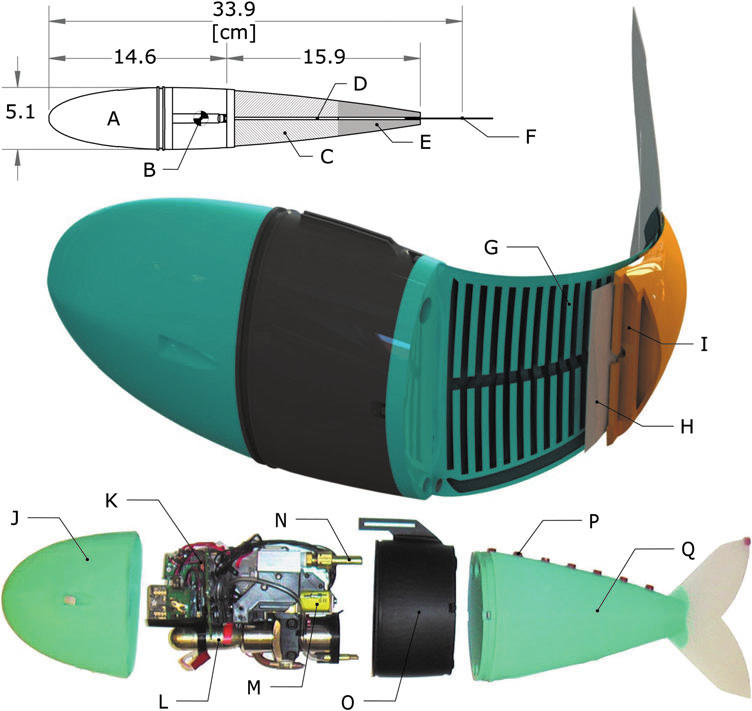
\includegraphics[width = 0.3\textwidth]{Figures/Introduction/fish.jpg}
    \caption{From left to right. Bionic Handling Assistant inspired by the trunk of an elephant \cite{BHA}. Octopus-inspired robot able to move and manipulate a wide range of objects \cite{octopus}.Bio-inspired soft robot replicating movement of a fish \cite{marchese2014}.}
    \label{fig1:softexample}
\end{figure}

There are some major differences between soft robots and the common rigid robots. First, a classification between both can be made on the basis of the compliance of their underlying materials \cite{Bionics2008}. Generally, classic robots are  made of rigid metal beams, whereas soft robots are made from soft polymer materials. 
The building materials of the robot largely determine the kinematic redundancy of the robot. Since soft robots are inherently compliant, they can undergo large deformations during normal operation. As a result of this compliance, gravity and payload cause a distributed deformation throughout the entire system . This gives the robot theoretically an infinite amount of degrees of freedom. This leads to non-unique solutions for a given end-effector position in the three dimensional workspace. In other word, the soft robot can take infinitely many configurations that yield the same end-effector position. On the contrary, traditional robots are often kinematically non-redundant. This implies that each joint is used to control an additional degree-of-freedom. The soft robots redundancy allows operation in unstructured and changing environments. Their dexterity allows them to move around objects.

Robot actuation another major difference between the two robot types. Rigid robots are often linked by rotatory or prismatic joints. Each of these joints are mechanically actuated using electric motors. Soft robots are mainly actuated pneumatically or by using variable length tendons \cite{Rus2015}. A pneumatically actuated soft robot is is the Bionic Handling assistant \cite{rolf2012constant}, as shown in Figure (\ref{fig1:softexample}). This type of soft robots have inflatable channels that cause a desired deformation when applying pressure. An example of a tendon driven is robot is the elephant trunk's robot \cite{cieslak1999elephant}. This manipulator consists of eight elastic segments linked together by coil springs. Each segment is controlled by two pairs of strings. Servo or linear actuators are used to wind and unwind the strings, with that controlling the movement of the robot. Both actuation methods introduce additional dynamics that largely affect performance of the entire control system. 

Lastly, most soft robots do not allow to use conventional sensing mechanisms. For hard robots their joint design allows to incorporate encoders to measure rotation and other sensory devices. As a result, position sensing, and determining the robots kinematic configuration is relatively easy. For soft robots, the compliant and lightweight nature often prevents to integrate conventional sensors, such as encoders, strain gauges and inertial measurement units (IMU's) \cite{Rus2015}, \cite{Lee2017}. Alternative sensory techniques are often needed. These methods include for instance optical sensors and stretch sensors based on macrobend fibres \cite{Sareh2015}.

\subsection{Control of soft robots}

Previous section discussed the contrast between rigid robots and soft robots. It showed that soft actuators distinct themselves from traditional robots on three fronts. Their inherent soft body leads to a theoretical infinite degree system. Resulting in non-uniqueness of solutions given an end-effector position. The actuation of soft robots introduces additional dynamics caused by the actuators. Furthermore, conventional sensory mechanism can often not be applied to soft robots, and therefore demand more complex sensory devices. These factors all effect the way soft robots can be controlled. Recent literature often tries to convey ready existing control theories and apply those to soft robotics.

The work of Thuruthel et al.(2018) \cite{george2018control} presents an overview of recent findings in soft robotic control for pneumatic actuated and tendon-driven soft robots. In this work, three control approaches are distinguished, namely, model-free, hybrid and model-based control. A model free control strategy does not use any kind of kinematic or dynamical description in its control approach. Instead, it exploits learning-based algorithms to dynamically control the robotic system. Hybrid controllers combine learning or empirical elements with a model-based approach. The model-based controllers rely on a analytical description of robotic system. Furthermore, for each control approach, a sub-division between kinematic and dynamical control is made. Here, kinematic control is defined as a zero order input-output relation. A change in input is directly observed in output, therefore this approach is lower-level compared to dynamical control. For the latter, the configuration space and/or task space variables' velocities are used in the control algorithm. 


Research conducted on the Bionic Handling Assistant (BHA), as shown in Figure \ref{fig1:softexample}, demonstrates that multiple control methods can be applied to the same robot. A model-free control approach was implemented in \cite{rolf2013efficient}. The inverse kinematics of the robot were obtained through machine learning, instead of model-derivation. Later work shows the implementation of a hybrid controller \cite{reinhart2017hybrid}. In this approach, an inverse kinematic model was used together with a learning model. Previous to this hybrid controller, a model-based controller was proposed by \cite{mahl2014bhakin}. However, this model-based controller only used a kinematic description of the soft robot. This research was followed up by \cite{falkenhahn2016dynamic}, which developed a dynamic controller. In this work the system is controlled with a nonlinear length controller based on feedback linearization. This controller was further supported by linear PD and feedforward control. 

In \cite{wang2013visual} visual servo control is used to control a cable-driven soft robotic manipulator. The manipulator, inspired by an octopus' tentacle, is shaped like a cone. On the outer surface of the soft robot four cables are uniformly distributed. These cables are on one end connected to the tip of the manipulator and on the other side connected to pulleys. By winding and unwinding the cables on the pulleys, the end-effector can be positioned in the task space. A kinematic-based visual servo controller is designed, based on linear PD feedback control with gravity compensation. Position sensing is done by a camera mounted at the tip of the robot, and a fixed feature point. Based on this visual information, a jacobian matrix is estimated, which is used in the kinematic controller.

In \cite{zhang2017visual} also visual servo control was implemented to control a tendon-driven soft robotic manipulator. Again, kinematic control is used for a reference tracking problem. Contrary to the previous research, where a jacobian matrix is estimated, here the jacobian is calculated by running a real-time FEM model parallel. A control architecture is set-up in which the reference input is ran through the FEM model, which outputs a jacobian and expected end-effector position. The jacobian is used in the controller to control the actual manipulator. The FEM model's expected end-effector position and actual end-effector position are used in a second controller to enhance jacobian estimation in the FEM model.

A model-based controller that uses a dynamical model in its control loop is presented in \cite{della2020model}. The robots infinite dimensionality is resolved by regarding the robot being composed of six individual actuatable segments. A Piecewise Constant Curvature (PCC) approach was used to describe the kinematics of the robotic actuator. For each segment Denavit-Hartenberg (DH) is used to describe the rigid robot equivalent, which is then used to derive a dynamic model. The proposed controller essentially is a computed torque controller with an additional PD controller. 

In aforementioned work, \cite{della2020model}, the infinite dimensionality of the soft robot is solved by assuming the robot consists of a fixed amount of segments. In this way the infinite dimensionality of the system can be approximated by fixed amount of degrees of freedom. This makes controller design easier. Of course, the reduction of degrees of freedom is at the cost of model accuracy. 




\section{Thesis outline and contribution}

The fundamentals of this research are provided in  \cite{Caasenbrood2020}, which developed a frame work to model the soft robot used in this work \hl{foto robot}. This soft robot also has a theoretical infinite degrees of freedom, as it is composed of flexible polymer. Furthermore it is pneumatically actuated, inducing additional dynamics into the control system, and a major limiting factor on achievable bandwidth. The sensing is done with inertial measurement unit (IMU) and an optical vision sensor. With this work we aim at developing a model-based control strategy for the pneumatically actuator planar soft robot to perform reference tracking problem. 

This thesis has the following structure. In Chapter ...

\hl{chapter 3}
\hl{chapter 4}
\hl{chapter 5}


Recapitulating, this thesis includes the following:


\begin{itemize}
    \item Development of a simplified non-linear dynamic model
    \item Parameter estimation
    \item Create a set-up for the planar soft robot 
    \item Development of a model-based control law
    \item Validation of the controller in experiments
\end{itemize}